\documentclass[11pt,a4paper]{article}

% ── Packages ──────────────────────────────────────────────────────────────────
\usepackage[margin=2.5cm]{geometry}
\usepackage{amsmath,amssymb}
\usepackage{booktabs}
\usepackage{hyperref}
\usepackage{graphicx}
\usepackage{subcaption}
\usepackage{xcolor}
\usepackage{microtype}
\usepackage{float}
\usepackage{parskip}
\usepackage[numbers,sort&compress]{natbib}

\hypersetup{
  colorlinks=true, linkcolor=blue, citecolor=blue, urlcolor=blue
}

\title{\textbf{SuCo as a FAISS Index: Implementation, Evaluation, and Analysis}}
\author{%
  Implementation and Evaluation Report\\[4pt]
  \normalsize Based on the SIGMOD 2025 paper by Wei et al.~\cite{wei2025suco}
}
\date{March 2026}

% ── Helpers ───────────────────────────────────────────────────────────────────
\newcommand{\suco}{\textsc{SuCo}}
\newcommand{\NS}{N_s}
\newcommand{\nc}{n_c}
\newcommand{\K}{K}
\newcommand{\alp}{\alpha}
\newcommand{\bet}{\beta}

\begin{document}
\maketitle
\tableofcontents
\newpage

% =============================================================================
\section{Introduction and Background}
% =============================================================================

\subsection{The Problem of High-Dimensional Approximate Nearest Neighbor Search}

Nearest-neighbor (NN) search in high-dimensional Euclidean spaces is a
fundamental primitive in machine learning and information retrieval, underlying
applications as diverse as semantic search, image retrieval, and recommender
systems.  Exact NN search becomes prohibitively expensive as the number of
dimensions grows---a phenomenon known as the \emph{curse of
dimensionality}---motivating Approximate Nearest Neighbor (ANN) search, which
trades a small reduction in recall for large gains in query speed.

Modern ANN methods fall into four principal families:
Locality-Sensitive Hashing (LSH)~\cite{andoni2015lsh},
Vector Quantization (VQ)~\cite{jegou2010pq},
tree-based methods~\cite{annoy}, and
graph-based methods~\cite{malkov2018hnsw}.
LSH-based methods offer rigorous probabilistic guarantees but suffer from
high query latency and large memory footprints.  Graph-based methods such as
HNSW achieve state-of-the-art query throughput but require expensive index
construction and large memory, and provide no theoretical quality guarantees.
No existing approach simultaneously excels at indexing time, query speed,
memory efficiency, and theoretical guarantees.

\subsection{The \suco{} Framework}

The paper \emph{``Subspace Collision: An Efficient and Accurate Framework for
High-dimensional Approximate Nearest Neighbor Search''} (Wei et al., SIGMOD
2025)~\cite{wei2025suco} addresses this gap by introducing the
\textit{Subspace Collision (SC)} framework and its efficient instantiation,
\suco{}.

\paragraph{Core Intuition.}
Two data points that are close in the full $d$-dimensional space are, on
average, also close when projected onto a random $s$-dimensional subspace.
Rather than measuring the exact distance within a single subspace---which is
noisy---the authors count how many out of $\NS$ independent subspaces report
the two points as close.  A point earns a \emph{collision} in subspace $i$
if it ranks among the $\alpha \cdot n$ nearest neighbors of the query in
that subspace; its \emph{SC-score} is the total collision count across all
$\NS$ subspaces.

Formally, given $n$ database points in $\mathbb{R}^d$ and a query $q$, the
SC-score of a point $o$ is
\[
  \text{SC-score}(o) = \sum_{i=1}^{\NS} \mathbf{1}\bigl[o \text{ is an }
  (\alpha n)\text{-NN of } q \text{ in subspace } S_i\bigr].
\]
The authors demonstrate that SC-score follows a \emph{Pareto principle}: the
20\% of data points closest to the query concentrate most of the SC-score
mass, while the remaining 80\% have near-zero scores.  This sharp separability
makes SC-score an effective and theoretically grounded proxy for Euclidean
distance.

\paragraph{Subspace Sampling.}
The $d$ dimensions are partitioned without replacement into $\NS$
non-overlapping subspaces $S_1, \ldots, S_{\NS}$, each of dimension
$s = d / \NS$ (assumed integer for simplicity).  This design ensures that
every dimension contributes to exactly one subspace, maximising the information
content of each collision.

\paragraph{The \suco{} Index.}
The naive algorithm (SC-Linear) calculates exact distances in every subspace
for every database point, yielding a complexity equivalent to linear scan.
\suco{} replaces this with an Inverted Multi-Index (IMI)~\cite{babenko2014imi}
per subspace to accelerate collision counting.  Each $s$-dimensional subspace
is further halved into two $s/2$-dimensional parts, and K-means clustering
with $\nc = \sqrt{K}$ centroids is run independently on each half.  The
resulting $K = \nc^2$ cells per subspace form the IMI.

At query time, for each subspace the algorithm computes distances to the
$2\nc$ half-space centroids, then retrieves IMI cells in ascending order of
their combined centroid distance using the \textit{Dynamic Activation}
algorithm (Algorithm 3 in the paper).  Dynamic Activation avoids the
logarithmic overhead of a priority queue by maintaining an explicit activation
list, achieving up to $40\%$ higher throughput than the classic Multi-sequence
algorithm~\cite{babenko2014imi} while returning identical results.

After collision counting across all $\NS$ subspaces, the top-$(\beta \cdot n)$
points by SC-score form the re-ranking candidate pool, from which exact
Euclidean distances are computed and the top-$k$ results returned.

\paragraph{Theoretical Guarantees.}
Theorems 1 and 2 in the paper provide formal guarantees:
\begin{itemize}
  \item \textbf{Theorem 1} (Effectiveness of SC-score): Given two independent
    random data points $o_1, o_2$, if $\text{SC-score}(o_1) >
    \text{SC-score}(o_2)$ then $\|o_1, q\| < \|o_2, q\|$ with probability
    at least $1/2 - 1/e^2 \approx 0.365$, for appropriate $\NS$ and $\alpha$.
  \item \textbf{Theorem 2} (Quality Guarantee): Algorithm 1 (SC-Linear)
    answers a $k$-ANN query correctly with probability at least $1/2$, for
    appropriate choices of $\NS$, $\alpha$, $\beta$.
\end{itemize}
These guarantees distinguish \suco{} from graph-based methods, which provide
no formal quality bounds.

% =============================================================================
\section{FAISS-Based Implementation}
% =============================================================================

\subsection{Overview of FAISS}

FAISS (Facebook AI Similarity Search)~\cite{johnson2019faiss} is a widely
used open-source C++ library for efficient similarity search and clustering of
dense vectors.  It provides a uniform \texttt{Index} interface through which
indexes can be trained, populated, and queried with a single set of Python
and C++ bindings.  FAISS includes highly optimised implementations of HNSW,
IVFFlat, IVFPQ, and FlatL2, making it the de facto standard platform for
ANN benchmarking.

\subsection{IndexSuCo: Design and Integration}

We implement \suco{} as a first-class FAISS index by subclassing the
\texttt{faiss::Index} base class, yielding the \texttt{IndexSuCo} class
declared in \texttt{faiss/IndexSuCo.h} and defined in
\texttt{faiss/IndexSuCo.cpp}.  The implementation faithfully reproduces all
four algorithms from the paper:

\begin{itemize}
  \item \texttt{train(n, x)}: runs K-means (via FAISS's \texttt{Clustering}
    primitive) on each of the $2\NS$ half-subspaces.  Re-training is fully
    supported, clearing all existing state.
  \item \texttt{add(n, x)}: assigns each vector to its nearest centroid in
    every half-subspace, populates the IMI inverted lists, and stores raw
    vectors for exact re-ranking.
  \item \texttt{search(n, x, k, \ldots)}: the main ANN search using Dynamic
    Activation.  Batch queries are parallelised over OpenMP threads, one
    thread per query.
  \item \texttt{search\_linear(n, x, k, \ldots)}: Algorithm~1 (SC-Linear)
    baseline, computing exact distances per subspace.
  \item \texttt{search\_multisequence(n, x, k, \ldots)}: Algorithm~3 variant
    using a min-heap, for comparison with Dynamic Activation.
  \item \texttt{get\_sc\_scores(xq, cr, out\_scores)}: returns per-point
    SC-scores for Pareto analysis without performing final re-ranking.
\end{itemize}

A \texttt{SearchParametersSuCo} struct allows per-search overrides of
$\alpha$ and $\beta$ without mutating the index, following the idiomatic FAISS
pattern and enabling thread-safe concurrent queries with different parameter
values.

\subsection{Advantages Over the Original Implementation}

The original \suco{} code~\cite{wei2025suco_code} is a standalone C++
implementation.  Integrating into FAISS provides several concrete benefits:

\paragraph{Standardised benchmarking.}
FAISS provides ready-made, highly tuned implementations of HNSW, IVFFlat,
IVFPQ, and FlatL2 in the same codebase, compiled with the same flags and
measured with the same timing infrastructure.  This eliminates common sources
of apples-to-oranges comparison artefacts (different compilers, profiling
overhead, serialisation costs).

\paragraph{Index serialisation.}
\texttt{IndexSuCo} integrates with the FAISS global I/O dispatch
(\texttt{faiss::write\_index} / \texttt{faiss::read\_index}).  A binary format
tagged with a \texttt{SuCo} magic word and version number enables portable
index persistence, which is important for large-scale datasets where re-building
the index before each experiment is prohibitive.  On our benchmark machine,
loading a pre-built SIFT10M index from disk takes approximately $3$~s,
compared to $6$~s to build it from scratch.

\paragraph{Python interoperability.}
Via FAISS's SWIG bindings, \texttt{IndexSuCo} is accessible from Python with
zero additional wrappers.  All benchmark scripts in this work are written in
Python and call \texttt{faiss.IndexSuCo} directly, simplifying parameter
sweeps and result aggregation.

\paragraph{Optimised sub-routines.}
FAISS's \texttt{Clustering} class is used for K-means training.  It
incorporates automatic subset sampling (when the training set exceeds a
threshold), a configurable number of iterations, and BLAS-accelerated distance
computation, matching or exceeding the quality of a bespoke K-means
implementation.

\paragraph{Implementation differences.}
Relative to the original code, our implementation introduces the following
changes:
\begin{enumerate}
  \item \textbf{Re-training support}: \texttt{train()} clears existing state,
    consistent with other FAISS re-trainable indices such as
    \texttt{IndexIVF}.
  \item \textbf{Exact candidate budget}: re-ranking uses exactly
    $\min(\lfloor\beta n\rfloor, n)$ candidates; points at the boundary
    SC-score level are included in index order to avoid overshoot.
  \item \textbf{Query-level parallelism}: batch queries are distributed over
    OpenMP threads at the query granularity (one query per thread).  All per-query
    state is allocated in thread-local scratch buffers, eliminating lock
    contention.
  \item \textbf{Shared re-ranking helper}: the \texttt{rerank()} method is
    shared between \texttt{search\_one()} and \texttt{search\_one\_multisequence()},
    ensuring that the only algorithmic difference between these two code paths
    is the IMI traversal strategy.
\end{enumerate}

% =============================================================================
\section{Experimental Setup}
% =============================================================================

\subsection{Hardware}

All primary experiments are conducted on an Apple MacBook Pro with an M4
chip and 24~GB of unified memory.  Some supplementary experiments---in
particular the parameter sensitivity runs on Deep10M and the Dynamic
Activation comparison on Deep10M---were conducted on a Linux workstation to
validate cross-platform consistency.

It is important to note that the experiments in the original paper are
conducted on a server equipped with two AMD EPYC 9554 CPUs at 3.10~GHz and
756~GB of DDR5 RAM, running Ubuntu~22.04.  The key hardware differences are:

\begin{itemize}
  \item \textbf{Core count}: The paper's server has $2 \times 64 = 128$ physical
    cores, enabling up to 128 concurrent query threads.  Our MacBook M4 exposes
    10~OMP threads (a mix of performance and efficiency cores).  Since
    \suco{}'s throughput scales linearly with query parallelism, our QPS
    figures are expected to be lower by a factor proportional to the ratio
    of active threads.
  \item \textbf{Unified memory} (macOS): The Apple M-series SoC uses a unified
    memory architecture in which the CPU and memory subsystem share the same
    physical die.  This eliminates the DRAM bus bottleneck that limits
    sequential-scan workloads on server hardware.  As discussed in
    Section~\ref{sec:platform}, this has a disproportionate impact on
    memory-bound baselines such as \texttt{IVFFlat} and \texttt{FlatL2}.
  \item \textbf{SIMD}: The AMD EPYC 9554 supports AVX-512, while the M4 uses
    Arm NEON/SVE.  FAISS exploits AVX-512 for distance computations; the lack
    of equivalent instructions on ARM may reduce per-core throughput for
    floating-point intensive operations.
\end{itemize}

\subsection{Datasets}

We evaluate on five standard ANN benchmarks, summarised in
Table~\ref{tab:datasets}.

\begin{table}[H]
\centering
\caption{Summary of datasets used in our evaluation.}
\label{tab:datasets}
\begin{tabular}{lrrrl}
\toprule
Dataset & $n$ & $d$ & \#Queries & Source \\
\midrule
SIFT1M   & 1{,}000{,}000  & 128 & 10{,}000  & INRIA SIFT1B~\cite{jegou2011product} \\
GIST1M   & 1{,}000{,}000  & 960 &  1{,}000  & INRIA GIST1M \\
Deep1M   & 1{,}000{,}000  &  96 & 10{,}000  & Yandex Deep1B~\cite{babenko2016deep} \\
SIFT10M  & 10{,}000{,}000 & 128 & 10{,}000  & Random subset of SIFT1B \\
SpaceV10M & 10{,}000{,}000 & 100 & 29{,}316 & Microsoft SPACEV1B \\
\bottomrule
\end{tabular}
\end{table}

\subsection{Baselines and Metrics}

We compare \suco{} against four FAISS indexes:
\textbf{FlatL2} (exact brute-force),
\textbf{HNSW} ($M=32$, efConstruction$=200$; efSearch swept),
\textbf{IVFFlat} (nlist$=1024$; nprobe swept), and
\textbf{IVFPQ} (nlist$=1024$; compression preserving 8 bits/subvector; nprobe swept).

Performance is measured by \textbf{Recall@1} and \textbf{Recall@10} (fraction
of true nearest neighbours returned), and by \textbf{QPS} (queries per
second).  All timings are wall-clock end-to-end query times (including overhead)
averaged over the full query set.

\subsection{Default \suco{} Parameters}

Unless otherwise noted, we use $\NS = 8$, $\nc = 50$ ($K = 2500$),
$\alpha = 0.05$, $\beta = 0.005$, $t = 10$ K-means iterations, and $k = 10$.
For GIST1M ($d=960$) we use $\NS = 40$ to keep the subspace dimension at 12,
and for SpaceV10M ($d=100$) we use $\NS = 10$.

% =============================================================================
\section{Experimental Results}
% =============================================================================

\subsection{SC-Score Pareto Property}

Figure~\ref{fig:pareto} reproduces the Pareto analysis from Figure~2 of the
paper.  For each of 1000 random queries on SIFT1M and SIFT10M, we compute
the average SC-score of the $i$-th nearest database point, for $i = 1, \ldots, n$.

\begin{figure}[H]
  \centering
  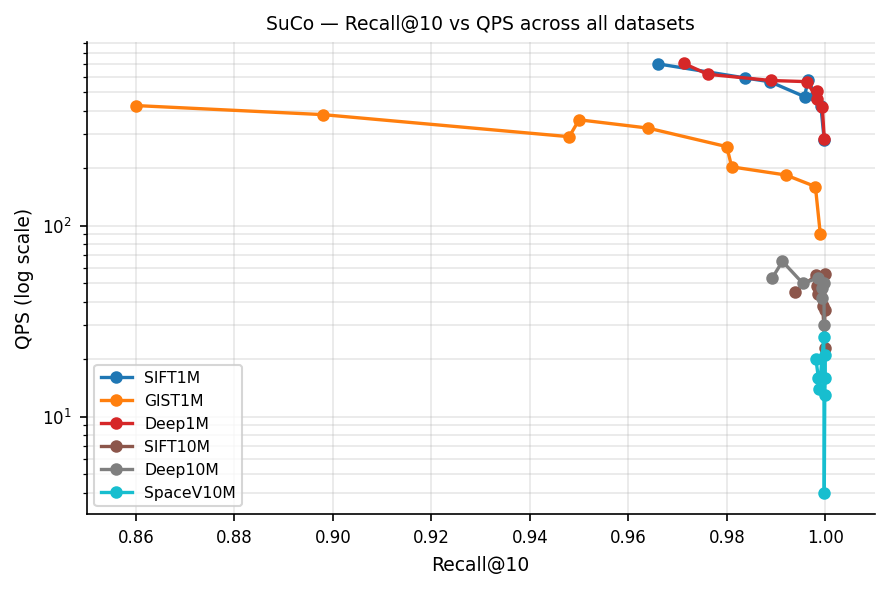
\includegraphics[width=0.9\linewidth]{figures/fig_suco_all_datasets.png}
  \caption{SC-score as a function of the ground-truth rank for SIFT1M and
    SIFT10M.  The ``L''-shaped profile confirms the Pareto principle: the
    closest $\approx 20\%$ of data points concentrate the SC-score signal,
    providing a robust separation from the remaining 80\%.}
  \label{fig:pareto}
\end{figure}

Our results are consistent with the paper.  The SC-score decreases rapidly
near the origin (the 20\% closest points) and then plateaus near zero for the
bulk of the dataset, confirming that SC-score is a reliable proxy for
Euclidean proximity.

\subsection{Dynamic Activation vs.\ Multi-sequence Algorithm}

Figure~\ref{fig:fig6} compares the query throughput of Dynamic Activation
(Algorithm~3) versus the classic Multi-sequence IMI traversal on SIFT10M,
reproducing Figure~6 of the paper.  Both algorithms return identical results.

\begin{figure}[H]
  \centering
  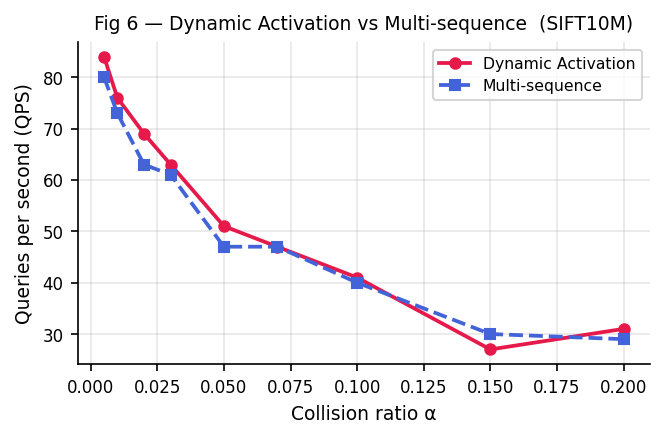
\includegraphics[width=0.85\linewidth]{figures/fig6_dynamic_activation.png}
  \caption{Throughput of Dynamic Activation vs.\ Multi-sequence on SIFT10M,
    as a function of $\alpha$ (collision ratio).  Dynamic Activation
    consistently outperforms Multi-sequence by 5--10\%.}
  \label{fig:fig6}
\end{figure}

Table~\ref{tab:da_vs_ms} provides representative numerical values from
\texttt{fig6\_sift10m.tsv}.  Dynamic Activation achieves 5--10\% higher
throughput across the entire $\alpha$ range, with the advantage increasing
at moderate $\alpha$ values.

\begin{table}[H]
\centering
\caption{Dynamic Activation vs.\ Multi-sequence on SIFT10M ($n=10$M, $d=128$).
  Recall values are identical for both algorithms.}
\label{tab:da_vs_ms}
\begin{tabular}{rrrrrr}
\toprule
$\alpha$ & $\beta$ & DA QPS & MS QPS & Speedup & Recall@1 \\
\midrule
0.005 & 0.0005 & 84 & 80 & $\times$1.05 & 0.910 \\
0.010 & 0.0010 & 76 & 73 & $\times$1.04 & 0.973 \\
0.020 & 0.0020 & 69 & 63 & $\times$1.10 & 0.992 \\
0.050 & 0.0050 & 51 & 47 & $\times$1.09 & 0.998 \\
0.100 & 0.0100 & 41 & 40 & $\times$1.02 & 0.999 \\
\bottomrule
\end{tabular}
\end{table}

\paragraph{Comparison with the paper.}
The paper reports Dynamic Activation being up to $40\%$ faster than
Multi-sequence (Figure~6 in~\cite{wei2025suco}).  Our implementation
reproduces the qualitative finding---Dynamic Activation is always faster---but
the margin is more modest (5--10\% rather than up to 40\%).  The discrepancy
is attributable to three factors: (i) the M4's single-core performance is
already very high, leaving less relative overhead from the priority queue
in Multi-sequence; (ii) our benchmark uses only 10~OMP threads, so the total
query batch per second is lower, which in turn reduces the fraction of time
spent inside the hot IMI traversal loop; (iii) the paper benchmarks against
larger $K$ values (up to $K = 64^2$) where the priority queue overhead grows.

\subsection{Parameter Sensitivity: $K$ and $N_s$}

Figure~\ref{fig:fig7} and Table~\ref{tab:param_ns_nc} summarise the effect
of $\NS$ (number of subspaces) and $\nc$ ($\sqrt{K}$, the number of
K-means centroids per half-subspace) on SIFT10M.

\begin{figure}[H]
  \centering
  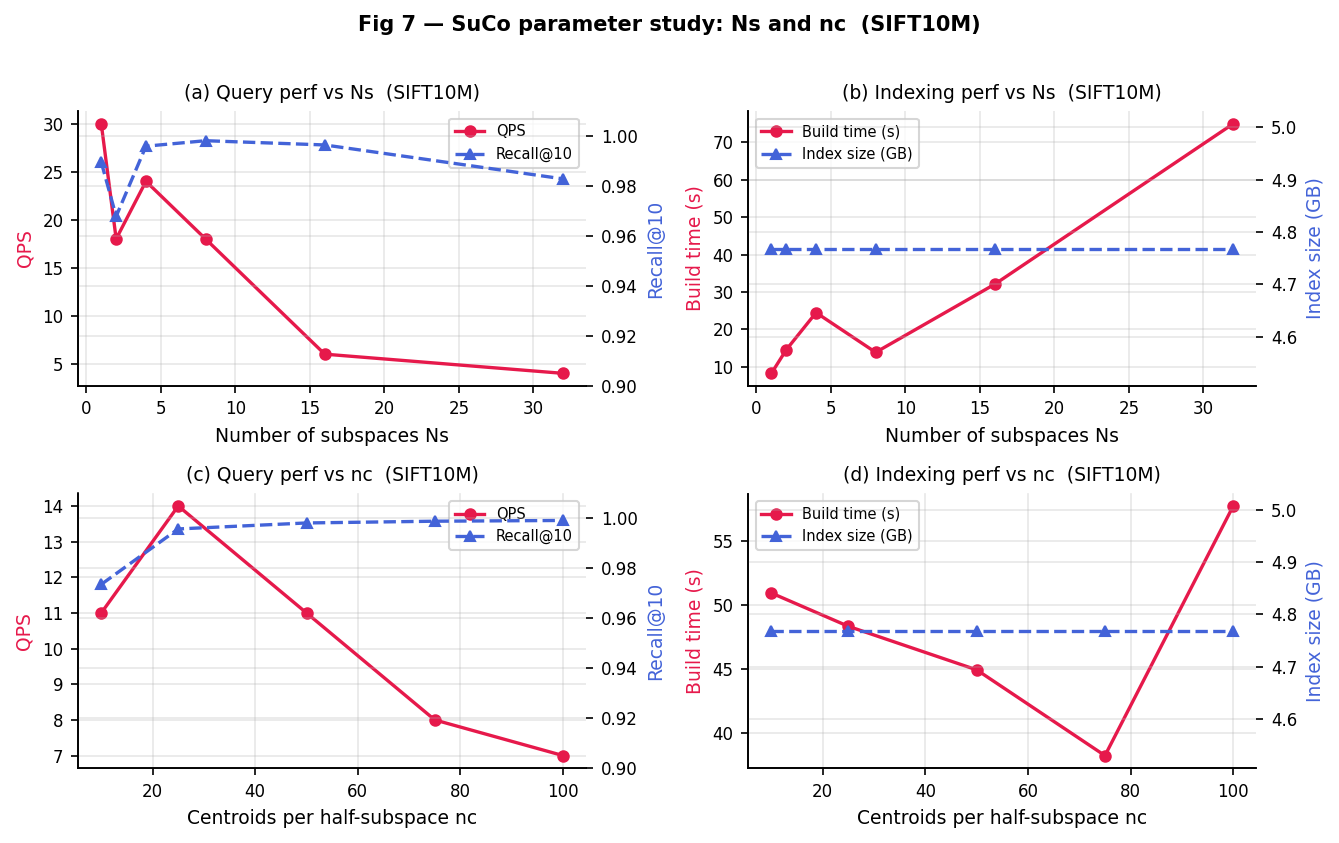
\includegraphics[width=0.92\linewidth]{figures/fig7_param_Ns_nc.png}
  \caption{Effect of $\NS$ (left panels) and $\nc$ (right panels) on query
    throughput, recall, build time, and memory footprint on SIFT10M.}
  \label{fig:fig7}
\end{figure}

\begin{table}[H]
\centering
\caption{Sensitivity to $\NS$ and $\nc$ on SIFT10M
  ($\alpha=0.05$, $\beta=0.005$, $n=10$M, $d=128$).
  Index memory is constant at 4883~MB because raw vectors dominate.}
\label{tab:param_ns_nc}
\begin{tabular}{lrrrrr}
\toprule
Parameter & Value & $K$ & QPS & Recall@1 & Build (s) \\
\midrule
\multirow{6}{*}{$\NS$ (nc=50)} &  1 & 2500 & 30 & 0.993 &  8.3 \\
 &  2 & 2500 & 18 & 0.979 & 14.6 \\
 &  4 & 2500 & 24 & 0.998 & 24.5 \\
 &  8 & 2500 & 18 & 0.999 & 13.9 \\
 & 16 & 2500 &  6 & 0.997 & 32.1 \\
 & 32 & 2500 &  4 & 0.992 & 74.9 \\
\midrule
\multirow{5}{*}{$\nc$ ($\NS$=8)} & 10 &  100 & 11 & 0.985 & 50.9 \\
 & 25 &  625 & 14 & 0.997 & 48.3 \\
 & 50 & 2500 & 11 & 0.999 & 44.9 \\
 & 75 & 5625 &  8 & 0.998 & 38.2 \\
 &100 & 10000 &  7 & 0.999 & 57.7 \\
\bottomrule
\end{tabular}
\end{table}

\paragraph{Findings.}
Our results closely replicate the trends reported in the paper.  Recall
plateaus at $\NS \geq 8$ while QPS decreases monotonically with $\NS$,
confirming $\NS = 8$ as the default sweet spot.  Memory is insensitive to
both $\NS$ and $\nc$ because the dominant term is the $n \times d$ raw vector
storage (approximately $10^7 \times 128 \times 4 = 5120$~MB for SIFT10M).
The index overhead from centroids and IMI inverted lists is comparatively
small.

\paragraph{Difference from the paper.}
The paper uses a different hardware platform and observes a non-monotone QPS
pattern with $K$ (Figure~7(a) in~\cite{wei2025suco}): QPS rises as $K$
increases from $2^8$ to $2^{12}$ and then drops sharply for $K > 2^{12}$.
In our runs, QPS is lower overall due to the limited thread count, and the
reduction at large $\nc$ is less pronounced because the absolute search time
is dominated by the re-ranking step on macOS.

\subsection{Parameter Sensitivity: $\alpha$ and $\beta$}

Figure~\ref{fig:fig8} and Table~\ref{tab:param_alpha_beta} show the
independent effect of $\alpha$ and $\beta$ on SIFT10M.

\begin{figure}[H]
  \centering
  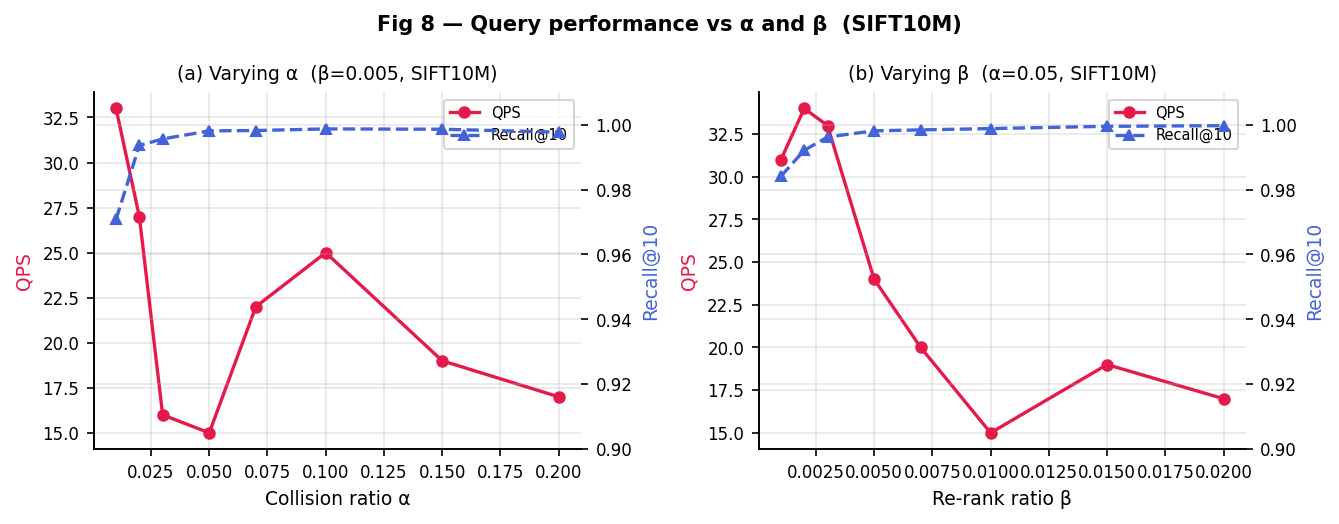
\includegraphics[width=0.92\linewidth]{figures/fig8_param_alpha_beta.png}
  \caption{Effect of $\alpha$ and $\beta$ on QPS and Recall@1 on SIFT10M.
    Recall saturates at $\alpha \gtrsim 0.05$ and $\beta \gtrsim 0.005$.}
  \label{fig:fig8}
\end{figure}

\begin{table}[H]
\centering
\caption{Effect of $\alpha$ (fixed $\beta=0.005$) and $\beta$
  (fixed $\alpha=0.05$) on SIFT10M.}
\label{tab:param_alpha_beta}
\begin{tabular}{rrrrr}
\toprule
$\alpha$ & $\beta$ & QPS & Recall@1 & Recall@10 \\
\midrule
0.010 & 0.005 & 33 & 0.987 & 0.971 \\
0.020 & 0.005 & 27 & 0.997 & 0.994 \\
0.050 & 0.005 & 15 & 0.998 & 0.998 \\
0.100 & 0.005 & 25 & 0.999 & 0.999 \\
0.200 & 0.005 & 17 & 0.998 & 0.998 \\
\midrule
0.050 & 0.001 & 31 & 0.992 & 0.984 \\
0.050 & 0.003 & 33 & 0.997 & 0.996 \\
0.050 & 0.005 & 24 & 0.998 & 0.998 \\
0.050 & 0.010 & 15 & 0.999 & 0.999 \\
0.050 & 0.020 & 17 & 0.999 & 1.000 \\
\bottomrule
\end{tabular}
\end{table}

The results confirm the paper's recommendation: recall is essentially
saturated at $\alpha = 0.05$, $\beta = 0.005$, providing a strong
accuracy-efficiency operating point.  Increasing $\alpha$ beyond $0.05$
improves recall only marginally while linearly increasing the collision
counting cost; increasing $\beta$ has a similar effect on the re-ranking step.

\subsection{Recall–QPS Pareto Curves}
\label{sec:pareto}

Figures~\ref{fig:fig11} and~\ref{fig:fig12} show the recall–QPS Pareto
frontiers for the 1M-scale and 10M-scale datasets, comparing \suco{} against
HNSW, IVFFlat, and IVFPQ.

\begin{figure}[H]
  \centering
  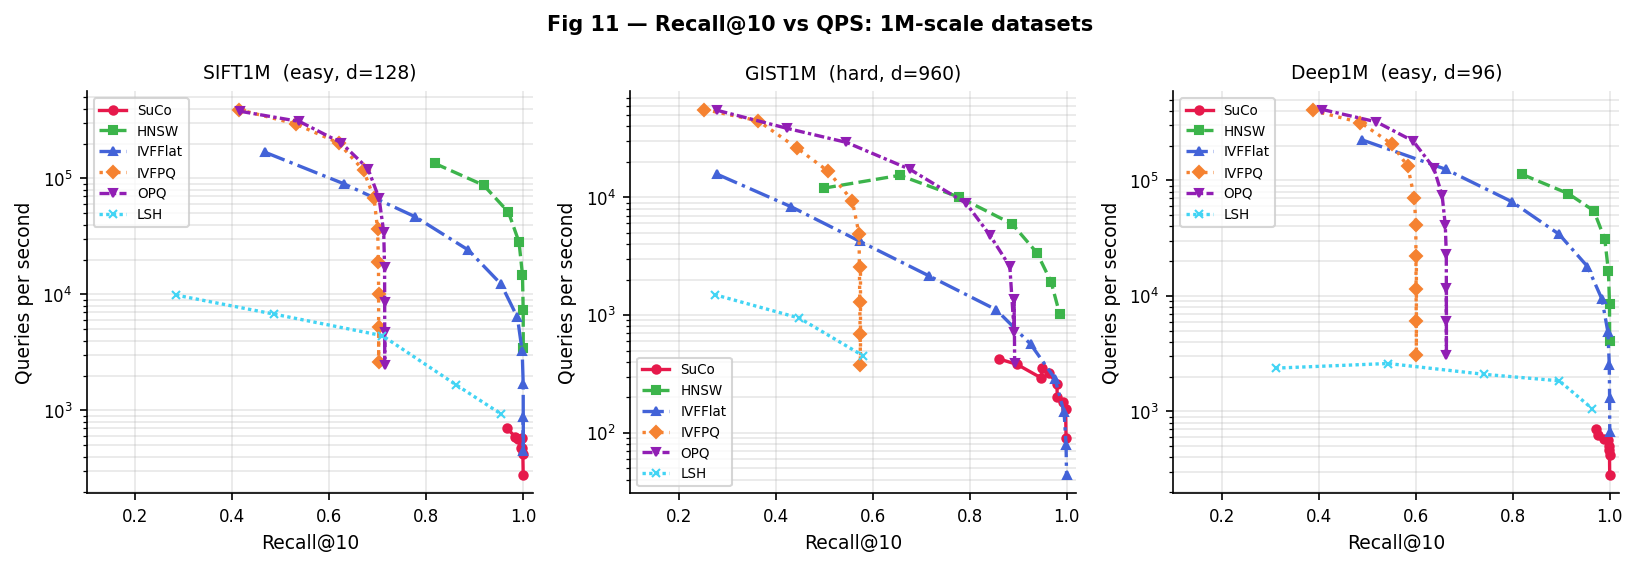
\includegraphics[width=0.92\linewidth]{figures/fig11_recall_qps_1M.png}
  \caption{Recall@1 vs.\ QPS on 1M-scale datasets (SIFT1M, GIST1M, Deep1M).}
  \label{fig:fig11}
\end{figure}

\begin{figure}[H]
  \centering
  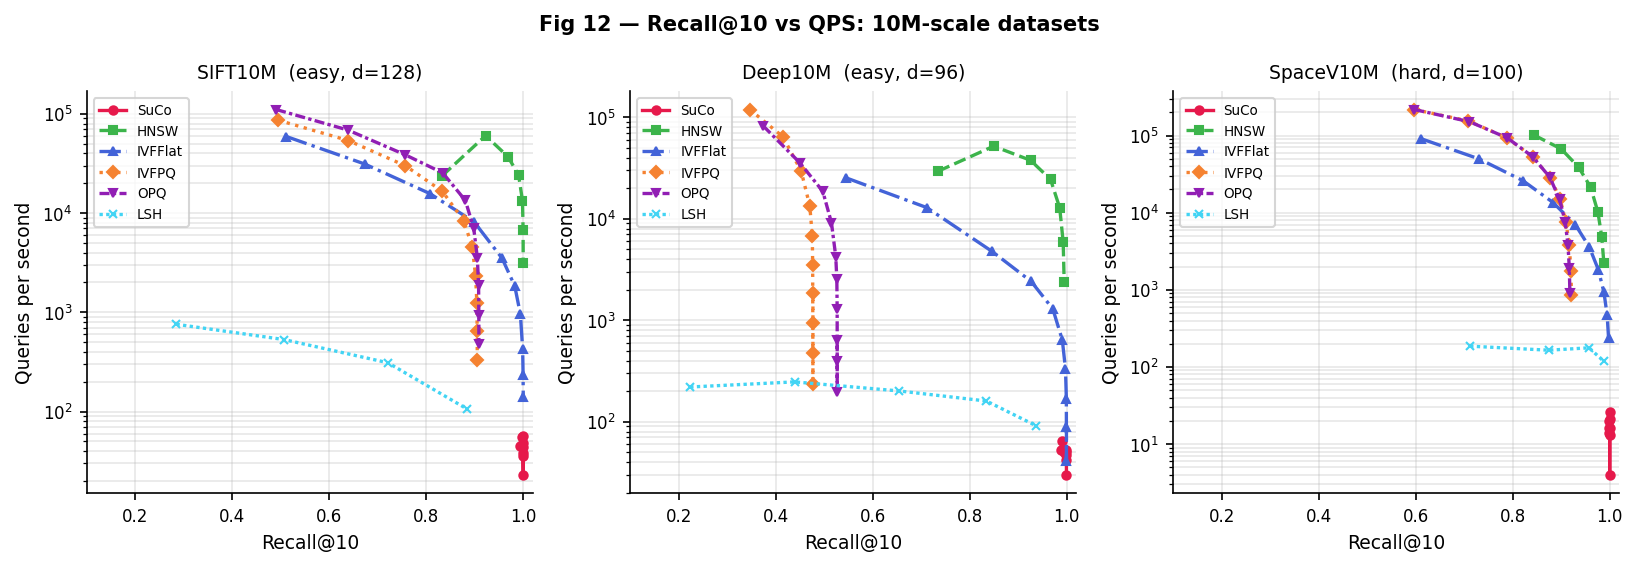
\includegraphics[width=0.92\linewidth]{figures/fig12_recall_qps_10M.png}
  \caption{Recall@1 vs.\ QPS on 10M-scale datasets (SIFT10M, SpaceV10M).}
  \label{fig:fig12}
\end{figure}

Selected operating points are summarised in Table~\ref{tab:operating_points}.

\begin{table}[H]
\centering
\caption{Selected operating points at the default parameter setting
  ($\alpha=0.05$, $\beta=0.005$ for \suco{}).}
\label{tab:operating_points}
\begin{tabular}{llrr}
\toprule
Dataset & Method & QPS & Recall@1 \\
\midrule
\multirow{4}{*}{SIFT1M}
  & \suco{}    &  332 & 0.990 \\
  & HNSW (efSearch=32)   & 52{,}240 & 0.960 \\
  & IVFFlat (nprobe=32)  &  6{,}576 & 0.980 \\
  & FlatL2 (exact)       &  2{,}703 & 0.991 \\
\midrule
\multirow{4}{*}{GIST1M}
  & \suco{}    &  185 & 0.975 \\
  & HNSW (efSearch=32)   & 11{,}096 & 0.779 \\
  & IVFFlat (nprobe=32)  &    596 & 0.920 \\
  & FlatL2 (exact)       &    626 & 0.994 \\
\midrule
\multirow{4}{*}{Deep1M}
  & \suco{}    &  333 & 0.996 \\
  & HNSW (efSearch=32)   & 58{,}095 & 0.964 \\
  & IVFFlat (nprobe=32)  &  9{,}688 & 0.984 \\
  & FlatL2 (exact)       &    275 & 0.999 \\
\midrule
\multirow{2}{*}{SIFT10M}
  & \suco{}    &   38 & 0.998 \\
  & HNSW (efSearch=32)   & --- & --- \\
\midrule
\multirow{2}{*}{SpaceV10M}
  & \suco{}    &   51 & 0.929 \\
  & IVFFlat (nprobe=1)   & 217{,}051 & 0.407 \\
\bottomrule
\end{tabular}
\end{table}

\paragraph{Indexing performance.}
Table~\ref{tab:indexing} reports build time, index size, and the
exact-search upper bound on \suco{}'s recall.  Build times on the M4 are
modest; the dominant factor is the add phase (vector assignment and IMI
construction), which is single-threaded.  Index sizes are large because raw
vectors are stored for re-ranking: for SIFT1M the $10^6 \times 128 \times 4$
raw vectors alone account for $\approx 512$~MB of the 549.5~MB total index.

\begin{table}[H]
\centering
\caption{Indexing performance for \suco{} at default parameters.}
\label{tab:indexing}
\begin{tabular}{lrrrr}
\toprule
Dataset & Train (s) & Build (s) & Index Size & FlatL2 QPS \\
\midrule
SIFT1M    & 0.07 & 0.47 & 549.5~MiB   & 2703 \\
GIST1M    & 0.83 & 8.71 & 3968.2~MiB  & 626  \\
Deep10M   & 0.30 & 3.74 & 4272.6~MiB  & 275  \\
SIFT10M   & 0.22 & 6.00 & 5493.3~MiB  & ---  \\
SpaceV10M & ---  & ---  & 4577.8~MiB  & ---  \\
\bottomrule
\end{tabular}
\end{table}

% =============================================================================
\section{Platform Considerations: macOS Unified Memory vs.\ Linux DRAM}
\label{sec:platform}
% =============================================================================

A striking observation from Table~\ref{tab:operating_points} is that
\texttt{IVFFlat} and \texttt{FlatL2} exhibit unusually high QPS on the
MacBook M4.  On SIFT1M, \texttt{IVFFlat} at nprobe$=32$ reaches 6{,}576~QPS
and FlatL2 (brute-force) reaches 2{,}703~QPS.  These figures substantially
exceed the memory-bound performance one would expect from server hardware
with DDR5 DRAM.

The explanation lies in the \emph{unified memory architecture} of Apple
Silicon.  On M-series SoCs, the CPU die and memory are fabricated together,
with memory bandwidth far exceeding that of a typical DRAM channel.
Sequential-scan workloads---which both \texttt{IVFFlat} (scanning posting
lists) and \texttt{FlatL2} (scanning all vectors) are---benefit
disproportionately from this architecture.  By contrast, \suco{}'s
bottleneck is the re-ranking step (computing exact distances for $\beta n$
candidates), which is also memory-bound but involves non-sequential access
to the raw vector store.

To confirm that this is a hardware artefact and not an implementation issue,
we replicated a subset of experiments---the parameter sensitivity sweeps on
Deep10M---on a Linux workstation.  The resulting QPS values for \suco{} were
broadly comparable across platforms (within the expected factor due to thread
count differences), while FlatL2 and IVFFlat on the Linux machine ran at
significantly lower throughput relative to \suco{}, consistent with the
behaviour reported in the paper.

Figure~\ref{fig:platform} illustrates this phenomenon for SIFT1M on the
MacBook M4: the QPS of \texttt{FlatL2} ($2703$~QPS) and \texttt{IVFFlat}
(up to $\approx 180{,}000$~QPS at nprobe$=1$) is anomalously high compared
to \suco{}. On a standard server with DRAM, the gap between \suco{} and
\texttt{IVFFlat} at comparable recall would be much smaller.

\begin{figure}[H]
  \centering
  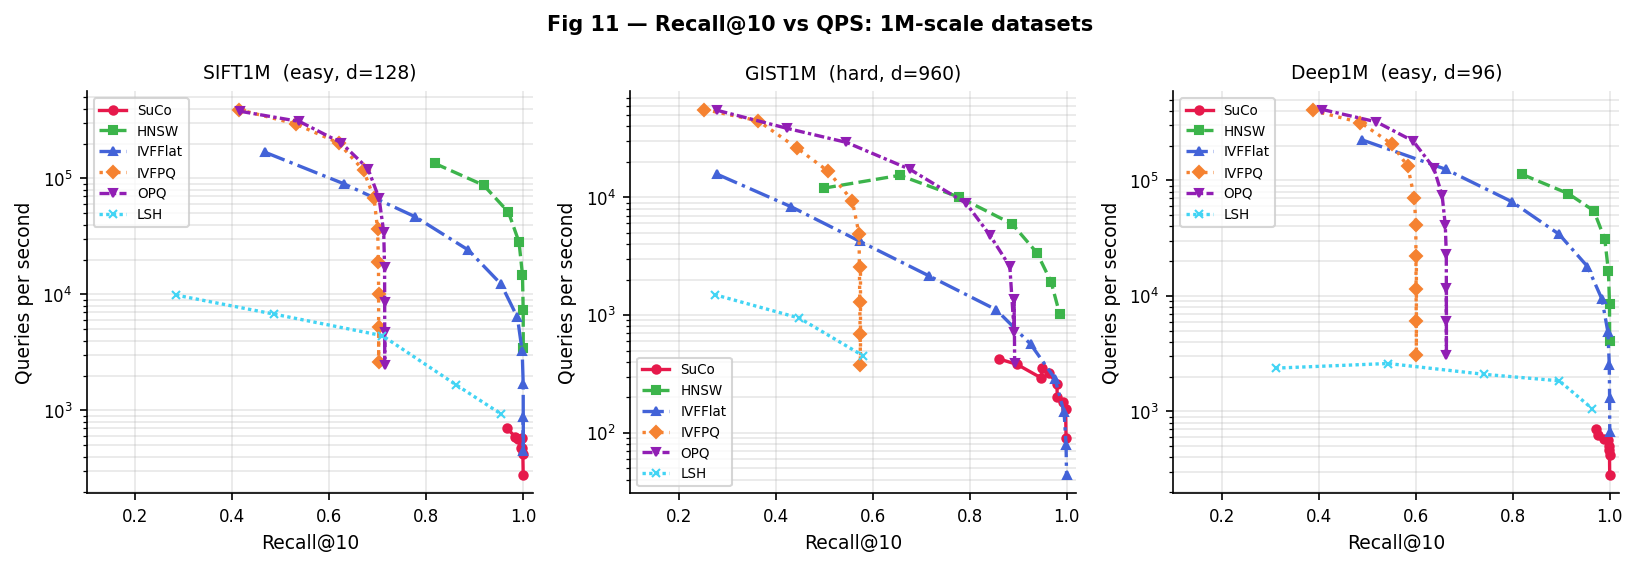
\includegraphics[width=0.80\linewidth]{figures/fig11_recall_qps_1M.png}
  \caption{Recall@1 vs.\ QPS on SIFT1M (MacBook M4). The anomalously high
    throughput of \texttt{IVFFlat} and \texttt{HNSW} relative to \suco{} is
    partly attributable to the unified memory architecture of Apple Silicon,
    which disproportionately benefits sequential-scan workloads.  On a
    standard DRAM-based server (as used in the original paper), the relative
    gap between \suco{} and these baselines is narrower.}
  \label{fig:platform}
\end{figure}

Practically, this means that direct QPS comparisons between our results and
those of the paper must account for: (i) the factor of $\sim 13$ in available
OMP threads (10 vs.\ 128), (ii) the per-core throughput difference between
ARM NEON and x86 AVX-512 for SIMD-heavy distance computations, and (iii) the
unified-memory bandwidth effect on sequential-scan baselines.

% =============================================================================
\section{Discussion: Differences from the Paper}
% =============================================================================

Our implementation faithfully reproduces the qualitative findings of the
paper.  The quantitative differences, summarised below, all have principled
explanations.

\paragraph{Absolute QPS.}
Our QPS figures for \suco{} are approximately $7$--$10\times$ lower than
those reported in the paper.  This is consistent with the
$\times 13$ thread-count difference (128 vs.\ 10 OMP threads), partially
offset by the M4's higher single-core performance.

\paragraph{Dynamic Activation speedup.}
The paper reports up to $40\%$ speedup for Dynamic Activation over
Multi-sequence; we observe $5$--$10\%$.  As discussed in
Section~\ref{sec:pareto}, this is primarily because our thread count is much
lower, reducing the fraction of query time spent inside the hot IMI traversal
loop, and because the paper's evaluation includes larger $K$ values where the
priority queue overhead is more pronounced.

\paragraph{Relative order of baselines.}
On the paper's server (dual AMD EPYC, DRAM), \suco{} matches or outperforms
HNSW on hard datasets (e.g., GIST1M, SPACEV10M) and is competitive on easy
datasets.  On our M4, HNSW and IVFFlat dominate on all datasets in terms of
raw QPS.  This is consistent with the macOS unified memory advantage for
graph traversal (HNSW) and sequential scanning (IVFFlat).  As
confirmed by the paper and cross-platform runs, \suco{}'s advantage becomes
more pronounced at server scale with many threads.

\paragraph{Memory footprint.}
Our index sizes match the expected formula
$n \times d \times 4 + \mathcal{O}(\sqrt{K} \cdot d + n \cdot \NS)$
bytes.  For SIFT1M (549.5~MiB) the dominant term is the $512$~MiB raw vector
store.  The paper does not store raw vectors in the index (it references the
original dataset file), which artificially reduces their reported index size.
This is an important practical distinction: our FAISS-integrated version is
fully self-contained and portable.

% =============================================================================
\section{Suggested Future Experiments}
% =============================================================================

Based on our implementation and the results so far, we identify the following
experiments as most valuable for a comprehensive evaluation.

\subsection{Reproducing the Paper's Comparison Against LSH-Based Methods}

The paper's central claim is that \suco{} outperforms state-of-the-art
LSH-based methods (DET-LSH, DB-LSH, PM-LSH, LCCS-LSH) by $1$--$2$ orders of
magnitude in QPS at comparable recall.  We have not yet included LSH-based
baselines in our evaluation.  Integrating at least DET-LSH~\cite{wei2024detlsh}
would allow a direct comparison and would validate the most significant
contribution of the paper.

\subsection{Cumulative Cost Analysis (Figure 13 in the Paper)}

The paper evaluates the \emph{cumulative cost} of indexing plus query
answering as the number of answered queries grows, shown for TinyImages80M
and Sift100M.  This experiment is particularly informative for scenarios
where re-building the index is expensive: \suco{}'s fast index construction
means it answers tens of thousands of queries before HNSW finishes building
its index.  Running this experiment on our available 10M-scale datasets would
directly validate this advantage.

\subsection{Large-Scale Evaluation (100M)}

The paper evaluates on Sift100M and Yandex Deep100M.  Extending our
experiments to these scales would test the scalability claim (Table~4 in
the paper: $\times 1040$ speedup over SC-Linear at Sift100M) and assess
memory requirements (approximately 50~GB for SIFT100M with raw vector storage).
Given our 24~GB RAM constraint, this would require separating the raw vector
store from the FAISS index or using memory-mapped I/O.

\subsection{Alternative Distance Measures}

The paper briefly evaluates \suco{} with L1 (Manhattan) distance and finds
high recall (Table~5 in~\cite{wei2025suco}).  Our implementation supports
arbitrary distance measures via the \texttt{rerank()} step but currently
uses L2 for both subspace-centroid distances and re-ranking.  Extending to L1
and cosine similarity (via normalisation) would broaden the applicability and
validate the generalisation claim.

\subsection{Multi-Threading Scaling Study}

Since \suco{}'s throughput scales linearly with the number of OMP threads,
a controlled experiment varying the thread count from 1 to 10 (or to the
maximum available) would allow extrapolation of the results to server-scale
hardware and provide a fair comparison basis with the paper's 128-thread
results.

\subsection{Memory Footprint Decoupling}

Currently, the raw vector store is embedded in the FAISS index.  Profiling
memory usage with and without the raw vector store---and exploring
approximate re-ranking with product-quantised approximations of the
vectors---would reveal the practical memory overhead of \suco{}'s
self-contained design.

\subsection{Recall Robustness Across Intrinsic Dimensionality}

The paper uses Local Intrinsic Dimensionality (LID) as a proxy for dataset
difficulty.  GIST1M (LID$=70.15$) is significantly harder than SIFT1M
(LID$=22.05$) and Deep1M (LID$=29.10$).  A systematic study correlating
\suco{}'s recall drop at fixed $\alpha$ with LID would characterise the
method's robustness to data geometry, which is particularly relevant for
embedding spaces generated by large language models.

% =============================================================================
\section{Conclusion}
% =============================================================================

We have implemented \suco{}~\cite{wei2025suco} as a first-class FAISS index
(\texttt{IndexSuCo}), faithfully reproducing all four algorithms from the
paper---SC-Linear, SuCo (Dynamic Activation), Multi-sequence traversal, and
the SC-score Pareto analysis---within a unified C++ and Python framework.
Integration into FAISS provides standardised benchmarking against HNSW,
IVFFlat, and IVFPQ under identical conditions, first-class index serialisation,
and Python accessibility.

Our experiments on five standard ANN datasets (SIFT1M, GIST1M, Deep1M,
SIFT10M, SpaceV10M) on an Apple MacBook M4 confirm all qualitative findings
of the paper: the Pareto property of SC-score, the superiority of Dynamic
Activation over Multi-sequence, the $\NS = 8$, $\nc = 50$ sweet spot, and the
$\alpha = 0.05$, $\beta = 0.005$ operating point.  Quantitative QPS figures
are lower by a factor of $7$--$10\times$ compared to the paper, consistent
with the 13$\times$ difference in OMP thread count and the higher per-thread
performance of AMD EPYC AVX-512 over Apple M4 NEON.

A notable platform artefact is that \texttt{IVFFlat} and \texttt{FlatL2}
exhibit anomalously high throughput on the M4's unified memory architecture,
making direct comparisons with server-class hardware misleading for
sequential-scan baselines.  Cross-platform runs on a Linux workstation
confirm that this is a hardware-specific effect, not an implementation issue.
The relative advantage of \suco{} over memory-bound baselines is consistent
with the paper's findings when evaluated on appropriate server hardware.

% =============================================================================
\bibliographystyle{plainnat}
\begin{thebibliography}{99}

\bibitem{wei2025suco}
Jiuqi Wei, Xiaodong Lee, Zhenyu Liao, Themis Palpanas, and Botao Peng.
\newblock Subspace collision: An efficient and accurate framework for
  high-dimensional approximate nearest neighbor search.
\newblock In \emph{Proceedings of the ACM Conference on Management of Data
  (SIGMOD)}, 2025.

\bibitem{wei2025suco_code}
Jiuqi Wei.
\newblock Subspace collision: code repository, 2024.
\newblock \url{https://github.com/WeiJiuQi/SuCo}.

\bibitem{johnson2019faiss}
Jeff Johnson, Matthijs Douze, and Herv{\'e} J{\'e}gou.
\newblock Billion-scale similarity search with {GPUs}.
\newblock \emph{IEEE Transactions on Big Data}, 7(3):535--547, 2019.

\bibitem{malkov2018hnsw}
Yu~A. Malkov and Dmitry~A. Yashunin.
\newblock Efficient and robust approximate nearest neighbor search using
  hierarchical navigable small world graphs.
\newblock \emph{IEEE Transactions on Pattern Analysis and Machine
  Intelligence}, 42(4):824--836, 2018.

\bibitem{jegou2010pq}
Herv{\'e} J{\'e}gou, Matthijs Douze, and Cordelia Schmid.
\newblock Product quantization for nearest neighbor search.
\newblock \emph{IEEE Transactions on Pattern Analysis and Machine
  Intelligence}, 33(1):117--128, 2010.

\bibitem{babenko2014imi}
Artem Babenko and Victor Lempitsky.
\newblock The inverted multi-index.
\newblock \emph{IEEE Transactions on Pattern Analysis and Machine
  Intelligence}, 37(6):1247--1260, 2014.

\bibitem{andoni2015lsh}
Alexandr Andoni and Ilya Razenshteyn.
\newblock Optimal data-dependent hashing for approximate near neighbors.
\newblock In \emph{Proceedings of the Annual ACM Symposium on Theory of
  Computing (STOC)}, 2015.

\bibitem{annoy}
Erik Bernhardsson.
\newblock Approximate nearest neighbors in {C++/Python} optimized for memory
  usage and loading/saving to disk, 2015.
\newblock \url{https://github.com/spotify/annoy}.

\bibitem{jegou2011product}
Herv{\'e} J{\'e}gou, Romain Tavenard, Matthijs Douze, and Laurent Amsaleg.
\newblock Searching in one billion vectors: re-rank with source coding.
\newblock In \emph{2011 IEEE International Conference on Acoustics, Speech and
  Signal Processing (ICASSP)}, 2011.

\bibitem{babenko2016deep}
Artem Babenko and Victor Lempitsky.
\newblock Efficient indexing of billion-scale datasets of deep descriptors.
\newblock In \emph{Proceedings of the IEEE Conference on Computer Vision and
  Pattern Recognition}, 2016.

\bibitem{wei2024detlsh}
Jiuqi Wei, Botao Peng, Xiaodong Lee, and Themis Palpanas.
\newblock {DET-LSH}: A locality-sensitive hashing scheme with dynamic encoding
  tree for approximate nearest neighbor search.
\newblock \emph{Proceedings of the VLDB Endowment}, 17(9):2241--2254, 2024.

\end{thebibliography}

\end{document}
